\documentclass[12pt]{article}

\usepackage[margin=1in]{geometry}
\usepackage{hyperref}
\hypersetup{
    colorlinks=true,
    linkcolor=blue,
    urlcolor=blue,
}
\usepackage{graphicx}
\usepackage{amsmath}
\usepackage{amssymb}
\usepackage[style=numeric, sorting=none]{biblatex}
\addbibresource{references.bib}

\title{Summary: Nanometer resolution imaging and tracking of fluorescent molecules with minimal photon fluxes}
\author{Ethan Rosenfeld}
\date{\today}

\begin{document}

\maketitle
\thispagestyle{empty}
\newpage

\tableofcontents
\newpage

\section{Motivation: resolution beyond the diffraction limit}
Microscopes are indispensable scientific instruments. Before their invention, humans accessed the information carried by electromagnetic radiation through the single-lens imaging system in the eye. The eye is limited to resolution of around 100 microns, so humans were unable to resolve fundamental biological structures like cells. A diffraction-limited optical microscope achieves resolution of $\lambda / 2 NA$, or around 200 nanometers. Since cells are around a few micrometers in size, optical microscopes can resolve sub-cellular structures such as the nucleus, mitochondria, and other organelles. 

Under typical bright-field illumination, many subcellular structures are indistinguishable, since contrast is low and structural information below the diffraction limit is lost. Fluorescence microscopy overcomes this barrier by labeling subcellular structures with fluorescent dyes and proteins. For example, the DAPI dye binds to DNA and enables visualization of DNA distribution in a cell, which for a eukaryotic cell labels the nucleus. A variety of fluorescent dyes have been developed for different labeling tasks, which has enabled breakthroughs in biological research. Concretely, fluorophores convey structural information (where are subcellular structures located/what is their shape) and quantitative information (how many molecules are present in a subcellular structure). Fluorescence microscopy also permits time-resolved imaging of dynamics in a cell such as ligand binding and diffusion processes.


\section{The diffraction limit}

A microscope is an imaging system which collects and magnifies light from a source onto a detector. A minimal microscope configuration is shown in Fig. \ref{fig:microscopes}a. In the case of fluorescence microscopy, the source may be a single fluorophore or collection of fluorophores. Light emitted from the source plane can be written as a sum of plane waves with wavevectors $\vec{k}_i$ and amplitudes $\tilde{E}(\mathbf{k})$ via the Fourier transform.

$$E(x,y) = \iint \tilde{E}(k_x, k_y)\, e^{i (k_x x + k_y y)} \, dk_x \, dk_y$$

\begin{figure}[h]
    \centering
    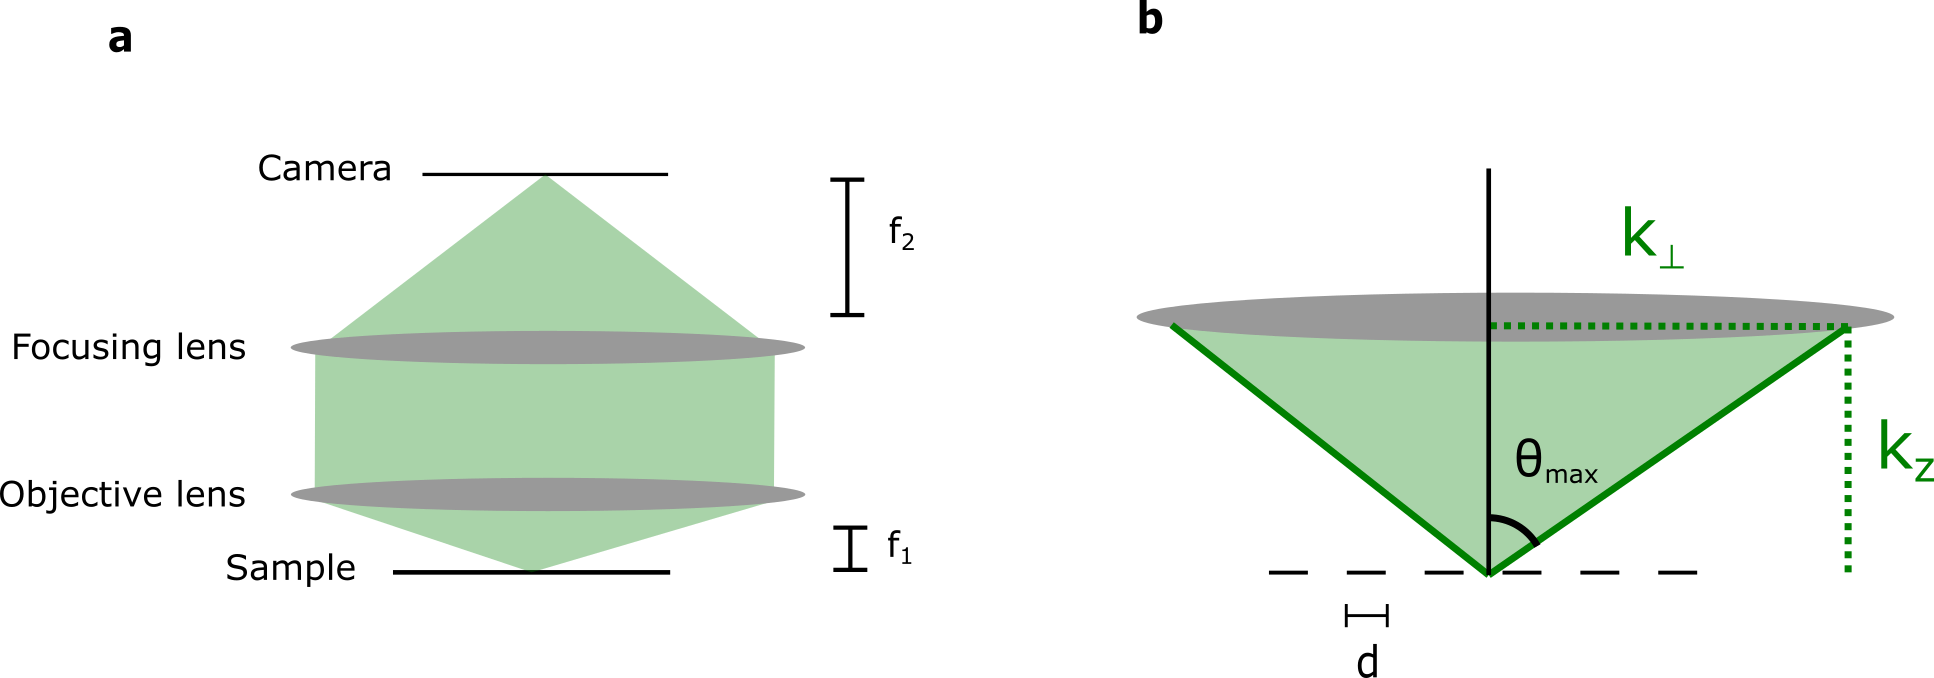
\includegraphics[width=\textwidth]{figs/fig_1.png}
    \caption{(a) An infinity-corrected microscope imaging system with a objective lens and a focusing lens. Light is directed from the source plane to be imaged on a camera. (b) A schematic of the light emitted by a bright sinusoidal grating with period $2d$. }
    \label{fig:microscopes}
\end{figure}

The effect of the objective lens is to collect all the light emitted into angles $\theta \leq \theta_{\text{max}}$. The transverse wavevector $k_\perp$ is related to the angle $\theta$ by $k_\perp = k \sin(\theta)$, where $k = \frac{2\pi}{\lambda}$ is the wavevector. Thus, the maximum transverse wavevector collected by the objective is $k_{\text{max}} = \frac{2 \pi NA}{\lambda}$, where $NA = n \sin(\theta_{\text{max}})$ is the numerical aperture. A sinusoidal grating with period $2d$ has a wavevector $k_{\text{grating}} = \frac{2\pi}{2d} = \frac{\pi}{d}$. Equating $k_{\text{grating}} = k_{\text{max}}$ gives the Abbe limit for resolution:
\[
d = \frac{\lambda}{2 n \sin(\theta_{\text{max}})}
\]

We can consider the effect of the frequency cutoff imposed by the objective lens as a pupil function $P(\mathbf{k})$. The pupil function is a binary function which is 1 inside the aperture and 0 outside and multiplies the fourier-domain fields as $$E(x,y) = \iint \tilde{E}(k_x, k_y)\, P(k_x, k_y)\, e^{i (k_x x + k_y y)} \, dk_x \, dk_y.$$

We can write the point spread function (PSF) as a fourier transform of the pupil function. For each fluorophore emitter, modeled as a delta function in the microscope source plane, we see a corresponding Airy-shaped PSF in the image plane. Through this, we see the another view of the resolution limit: that the ideal image is blurred out by convolution with the PSF.

\[
h(x,y)=\mathcal{F}^{-1}\{P(k_x,k_y)\}
\]

\begin{figure}[h]
    \centering
    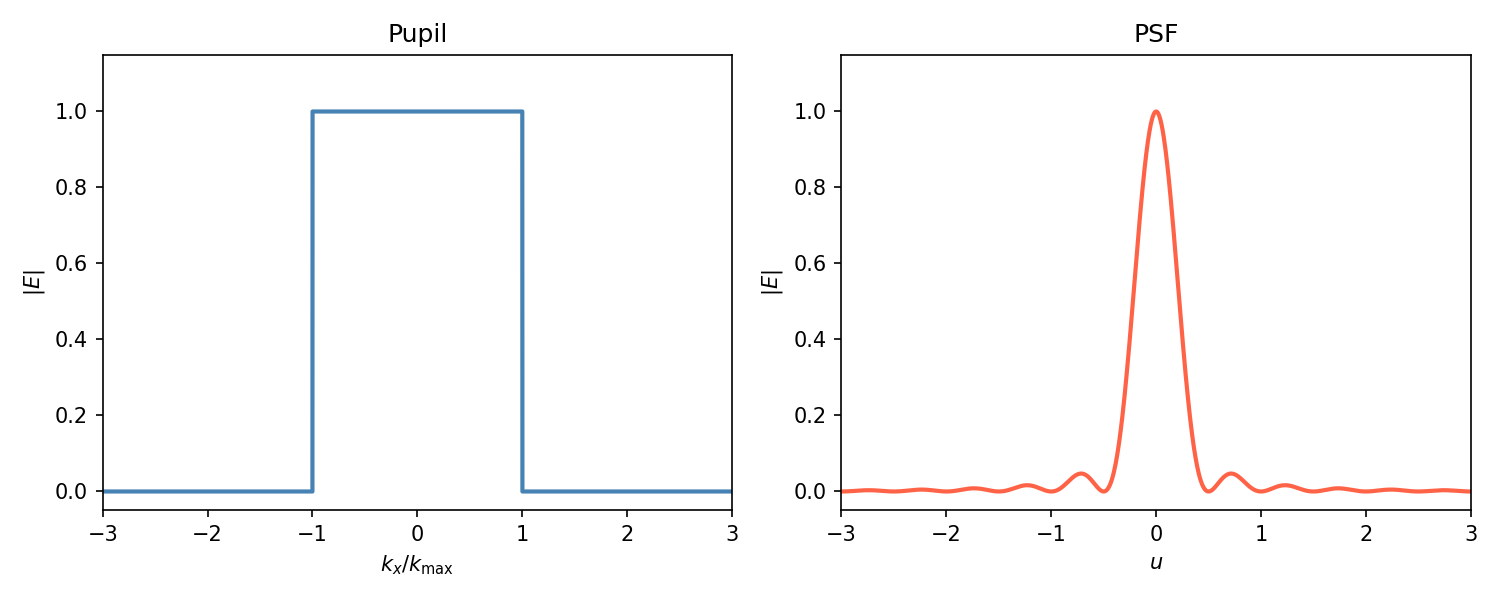
\includegraphics[width=\textwidth]{figs/fig_2.png}
    \caption{The pupil function in one dimension is shown as a frequency cutoff where $k_{x} = k_{\text{max}}$. The point spread function (PSF) is the fourier transform of the pupil function, appearing as a sinc function.}
    \label{fig:psf}
\end{figure}

\section{Super-resolution}

\subsection{Parameter estimation}

To discuss super-resolution, it is first helpful to discuss parameter estimation in the context of microscopy. In its simplest form, parameter estimation deals with a system which has a single parameter $\theta$ and a series of measurements which yield noisy data $\mathbf{X}$. The goal is to produce an estimate $\hat{\theta}$ of the parameter $\theta$ which is as close as possible to the true value $\theta$. It is possible to bound the error in the estimate $\hat{\theta}$ by the Cramér-Rao bound (CRB), which is a lower bound on the variance of the estimate. The CRB is defined as 
\[
\text{Var}(\hat{\theta}) \geq \frac{1}{F(\theta)}
\]
and the Fisher information is defined as
\[
F(\theta) = \mathbb{E}\left[\left(\frac{\partial \log p(\mathbf{X}|\theta)}{\partial \theta}\right)^2 \Big| \theta\right].
\]

In the context of localizing a single fluorophore emitter in the microscope source plane, the parameter of interest is the position of a fluorophore emitter $\vec r_0$. We can assume for the sake of simplicity that the fluorophore's PSF is isolated from other fluorophores. The microscope camera records photons as a function of position, $n(\vec r)$. For a fluorophore at the origin, the Cramér-Rao bound for the standard deviation of the estimate of the fluorophore's position can be derived to be $$\hat \sigma_{\text{CRB}}(0) = \frac{\sigma}{\sqrt{N}}$$ where $\sigma$ is the standard deviation of the PSF approximated as a Gaussian and $N$ is the total number of photons detected. For a realistic case of focusing a 650 nm laser though a $NA=1.4$ objective lens, the PSF approximated as a Gaussian has standard deviation width $\sigma = 100$ nm. So, for only 500 photons, the CRB for the position is $\hat \sigma_{\text{CRB}} = 4.5$ nanometers.

\subsection{Super-resolution techniques}

The localization precision of $<10$ nanometers is far below the diffraction limit, but challenging to achieve in practice due to the requirement that a single fluorophore is active at a time. The revolution in super-resolution in the early 2000's depended on clever photochemical techniques to engineer a situation where a collection of fluorophores clumped smaller than the PSF is active. These techniques fall into two categories, structured illumination and time-division multiplexing. Structured illumination is commonly implemented as Stimulated Emission Depletion (STED) microscopy, pioneered by Hell et al. \cite{hellBreakingDiffractionResolution1994} in 1994. Time-division multiplexing is commonly implemented as Stochastic Optical Reconstruction Microscopy (STORM), introduced by Rust et al. \cite{rustSubdiffractionlimitImagingStochastic2006} in 2006, and Photo-Activated Localization Microscopy (PALM), introduced by Betzig et al. \cite{betzigImagingIntracellularFluorescent2006} in 2006.

STORM uses random photochemical activation and deactivation of fluorescent dyes to cause stochastic blinking of fluorophores. Reconstruction of the fluorophore's position is done computationally in post-processing after recording a video of the emissions. PALM uses photoactivatable fluorescent proteins to cause photoactivation of widely spaced subsets of fluorophores followed by permanent deactivation. 

\subsection{Fluorophore blinking in STORM}

The STORM technique underlies the development of MINFLUX, the topic of the next section. In STORM, an excitation laser is used to induce fluorescence of fluorophores. Via a random photochemical process, the fluorophore undergoes a chemical reaction that brings it to a dark state where it cannot fluoresce. Fluorophores are re-activated by a reactivation, which induces the reverse chemical reaction to bring the fluorophore back to a fluorescent state. The intensities of the excitation and reactivation lasers define the on-off switching rates in a simplified rate-equation model \cite{heilemannSubdiffractionResolutionFluorescenceImaging2008} defined by
\[
\frac{dM_{\text{on}}}{dt} = k_{\text{on}} M_{\text{off}} - k_{\text{off}} M_{\text{on}},
\]
where $M_{\text{on}}$ is the number of fluorophores in the on state, $M_{\text{off}}$ is the number of fluorophores in the off state, $k_{\text{on}}$ is the on-rate, and $k_{\text{off}}$ is the off-rate. At steady state, this gives
\[
\frac{M_{\text{on}}}{M_{\text{total}}} = \frac{k_{\text{on}}}{k_{\text{on}} + k_{\text{off}}}
\]

By tuning the intensities of the excitation and reactivation lasers, the on-off switching rates can be controlled such that on average, only a single fluorophore is active at a time in a PSF-sized region of the source plane.

\section{MINFLUX}

\subsection{MINFLUX algorithm}

The MINFLUX (localization with MINimal photon FLUX) technique was introduced by Balzarotti et al. \cite{balzarottiNanometerResolutionImaging2017} in 2018. MINFLUX is an extension of STORM and thus based on stochastic blinking of fluorophores. However, MINFLUX departs from STORM in its method of localization. Whereas STORM uses camera localization, MINFLUX uses a moveable structured illumination pattern. In the end, MINFLUX achieves scaling of the Cramér-Rao bound with a length scale $L/4$ as $$\hat \sigma_{\text{CRB}} = \frac{L}{4\sqrt{N}},$$ where $L$ is an experimentally tunable parameter of the structured illumination pattern.

\begin{figure}[h]
    \centering
    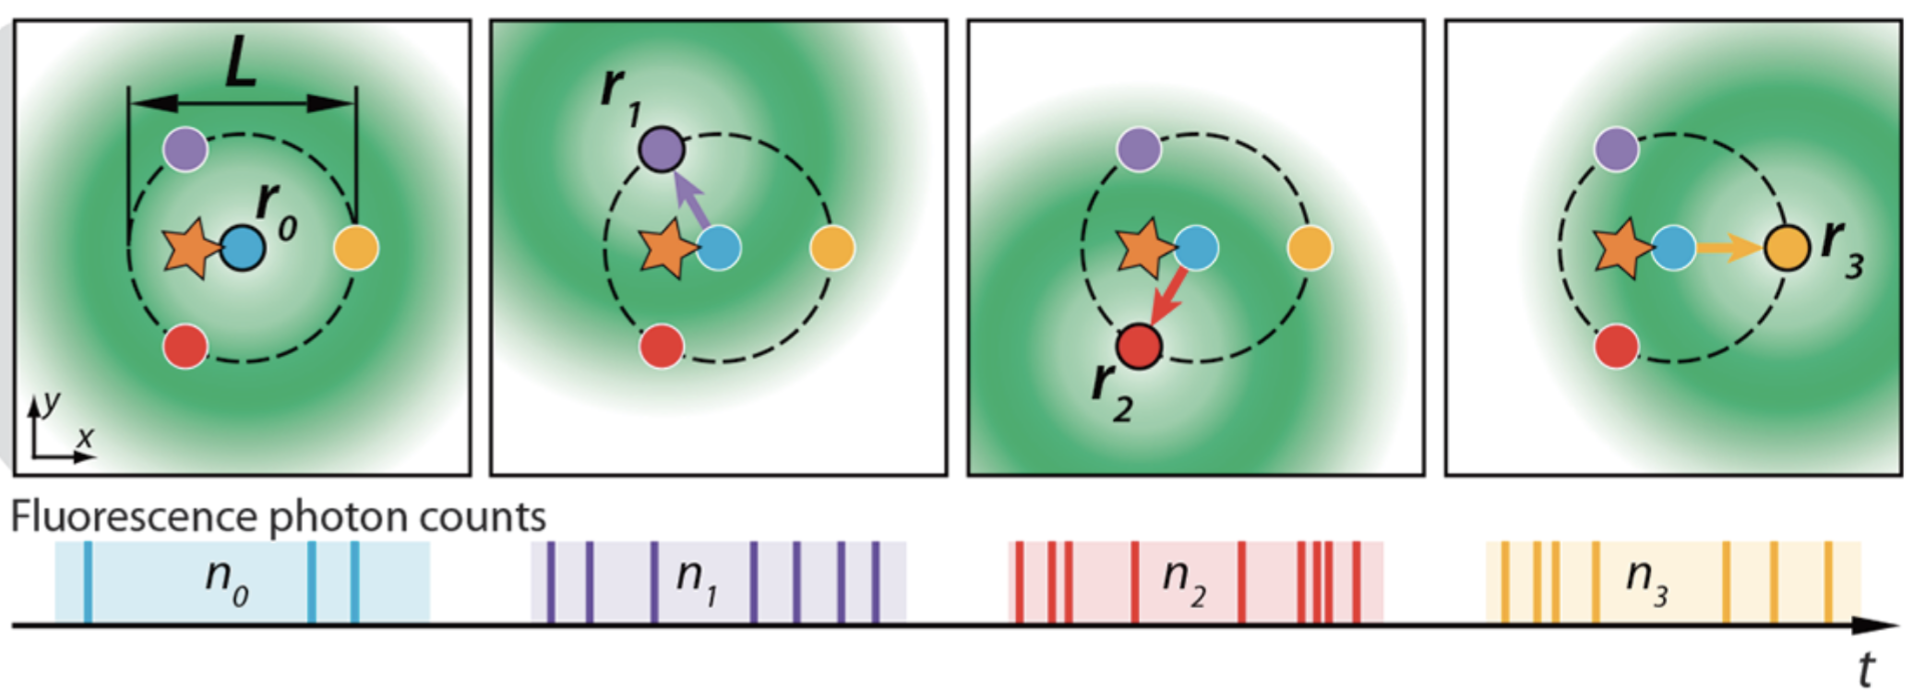
\includegraphics[width=\textwidth]{figs/fig_3.png}
    \caption{This is Fig. 2b from the MINFLUX paper.\cite{balzarottiNanometerResolutionImaging2017} The position of the fluorophore is shown as a star. The doughnut is moved sequentially through the list of positions $0 \rightarrow 1 \rightarrow 2 \rightarrow 1$. The photons emitted in each position are counted.}
    \label{fig:minflux}
\end{figure}

In practice, MINFLUX is implemented in 2 dimensions with a moveable doughnut-shaped pattern with an intensity minimum at the center. To localize a collection of flurophores spaced below the diffraction limit, the algorithm is implemented as follows:

\begin{enumerate}
    \item Localize a collection of fluorophores via conventional fluorescence microscopy. Estimate the centroid of the clump of fluorophores.
    \item Tune the excitation laser and reactivation laser such that on-average, only one fluorophore is active at a time in the region of the excitation pattern.
    \item During the imaging, rapidly cycle the excitation pattern over the 4 positions, time-tagging the photons emitted from the fluorophore at each excitation position.
    \item Determine isolated fluorophore emission events.
    \item In an isolated event, use the number of photons at each excitation position to estimate the position of the fluorophore.
\end{enumerate}

\subsection{MINFLUX applications}

In Balzarotti et al. \cite{balzarottiNanometerResolutionImaging2017}, MINFLUX was first used to localize a collection of fluorophores localized on a 2D grid of DNA origami with a spacing of 6 nanometers and 11 nanometers. To localize fluorophores on the 11 nm spaced DNA origami, the doughnut-shaped excitation pattern was cycled over a triangular pattern with $L=70$ nanometers. Only fluorophore emission events with more than 500 photons were used. The authors achieved an experimental localization precision of 2.1 nanometers for the 11 nanometer grid. On a 6 nanometer grid of DNA origami, the authors used $L=50$ nanometers and events with over 1000 photons to achieve a localization precision of 1.2 nanometers. Secondly, the authors used MINFLUX to record nano and microscale motion of fluorophores within a living E. coli bacterium. The photon efficiency of MINFLUX is exploited to track diffusion of fluorophores within the bacterium using an average of 9 photons per localization over the course of over 1000 localizations. The measurement permitted estimation of the diffusion constant $D$. 

\section{Conclusion}

MINFLUX appears to be a powerful tool that combines each of the best qualities of the previous generation of super-resolution microscopes: using both structured illumination and time-division multiplexing.  Moreover, the MINFLUX technique is readily implemented in existing microscopes and only requires commercially available optics. Although the MINFLUX technique was only developed 8 years ago, it has already enabled substantial advances in structural biology, used in dozens of papers published in the years since its invention. Deguchi et al. \cite{deguchiDirectObservationMotor} used MINFLUX to record 4 nanometer substeps of the motor protein kinesin-1 on microtubules. Schleske et al. \cite{schleskeMINFLUXRevealsDynein2024} used MINFLUX to record 8 nanometer steps of the dynein protein--responsible for intracellular transport. Sau et al. \cite{sauOverlappingNuclearImport2025} showed that MINFLUX can directly track single molecules through nuclear pores with nanometer precision, revealing that import and export occur in overlapping, highly confined pathways. MINFLUX achieves the long-standing goal of super-resolution microscopy: localization of individual fluorophores with a far-field microscope at room temperature.

\printbibliography

\end{document}
